% -----------------------------------------------------
% 		Creating a New Project
% -----------------------------------------------------
\section{Creating a New Project}

Creating a new project can be done by selecting \menupath{File, New Project...} from the menubar or by selecting the \textit{Create New Project} icon from the "Quick Start" menu, as shown in \figref{fig:vivadostartcreate}. \\


\begin{figure}
	\centering
	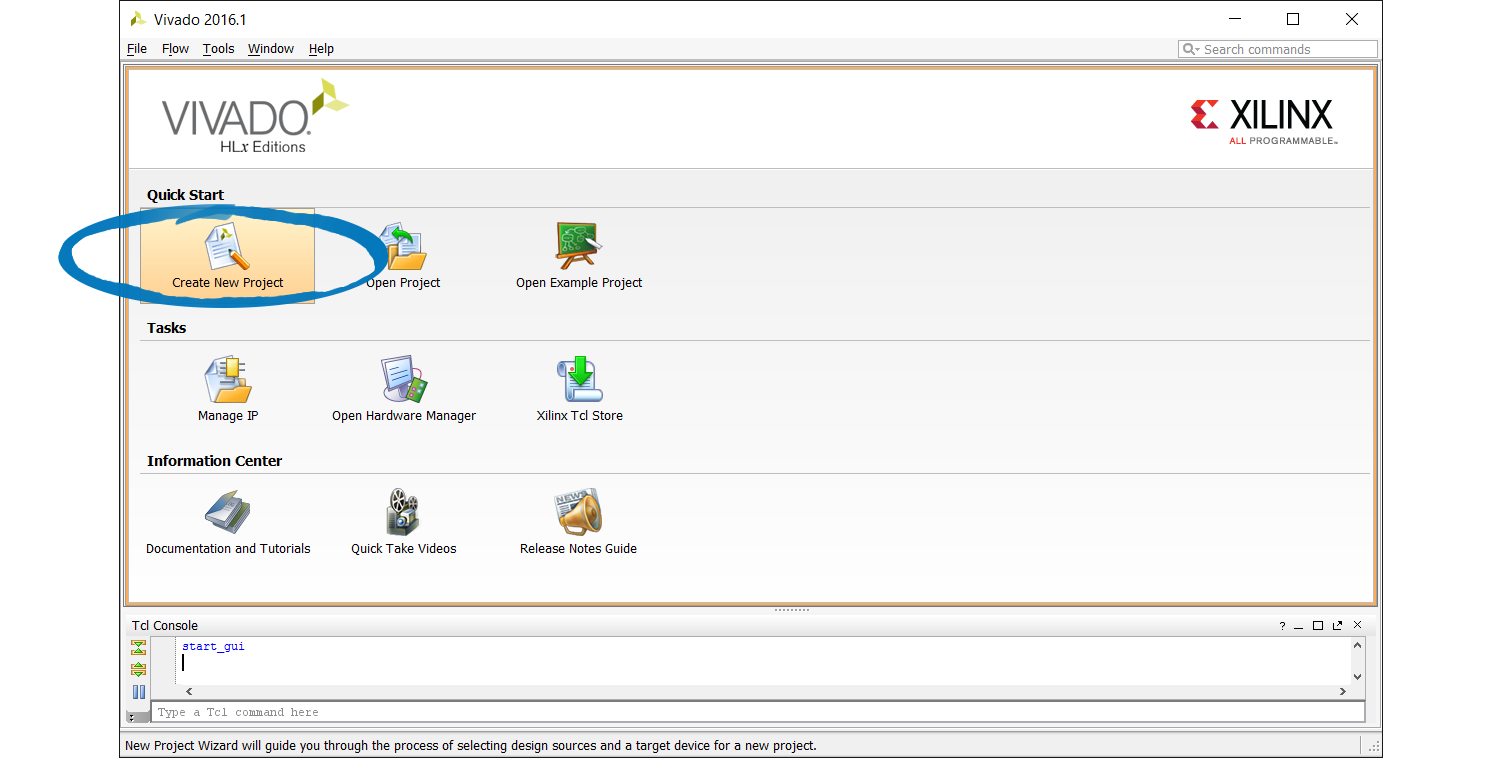
\includegraphics{images/vivado/create_new_project.png}
	\caption[Vivado Startup Create New Project]{Vivado Startup Create New Project}
	\label{fig:vivadostartcreate}
\end{figure}


~\\
The first step to creating a new Vivado project is to select the project name and parent directory. By default, Vivado will create a new subdirectory for which to store the project files. It is highly recommended that this setting be left unchanged to keep the project files and directories organized and easily accessible for development (\ie from the SDK). \figref{fig:vivadonewprojectname} shows the input of the project name and parent directory when creating a new project.


\begin{figure}
	\centering
	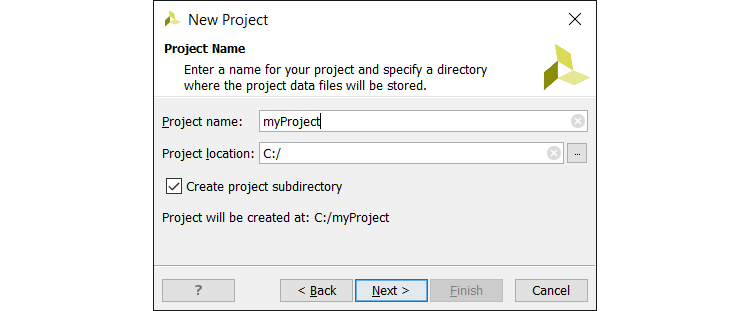
\includegraphics{images/vivado/new_project_name.png}
	\caption{Selecting Project Name and Parent Directory}
	\label{fig:vivadonewprojectname}
\end{figure}


%%%-------- Project Type and Sources ------------
\subsection{Project Type and Sources}
At this point in the project creation process, IP and design sources can be added to the project. If you would like to include existing sources, you will prompted to include those before choosing a project board. If you choose not to include any existing assets or constraints, the \menupath{Do no specify sources...} checkbox, shown in \figref{fig:newprojecttype}, can be selected to skip this step. Sources can be added to the project at any time after creation as outlined \hyperref[sub:addsources]{below}.

\begin{figure}
	\centering
	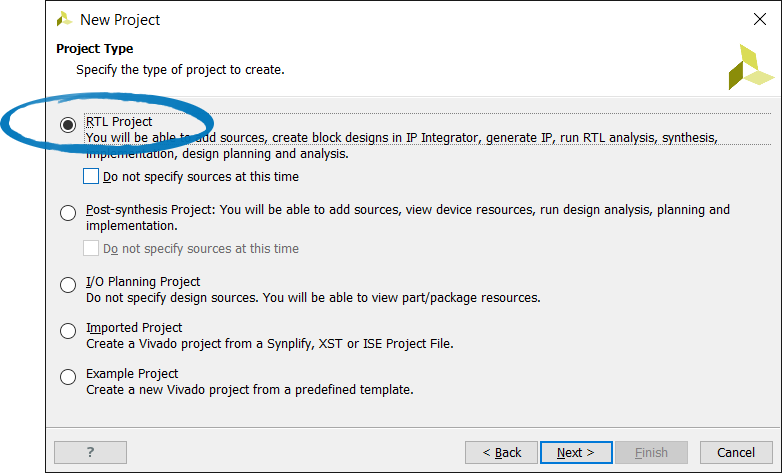
\includegraphics{images/vivado/new_rtl_project.png}
	\caption{Project Type Selection Dialog}
	\label{fig:newprojecttype}
\end{figure}


%%%-------- Choosing a Project Board ---------
\subsection{Choosing a Project Board}

If the board files have been copied and loaded properly, they will be listed in the table of boards. To view the available boards, choose "Boards" rather than "Parts" at the top of the window as shown in \figref{fig:vivadoprojectboard}. \\


\begin{figure}
	\centering
	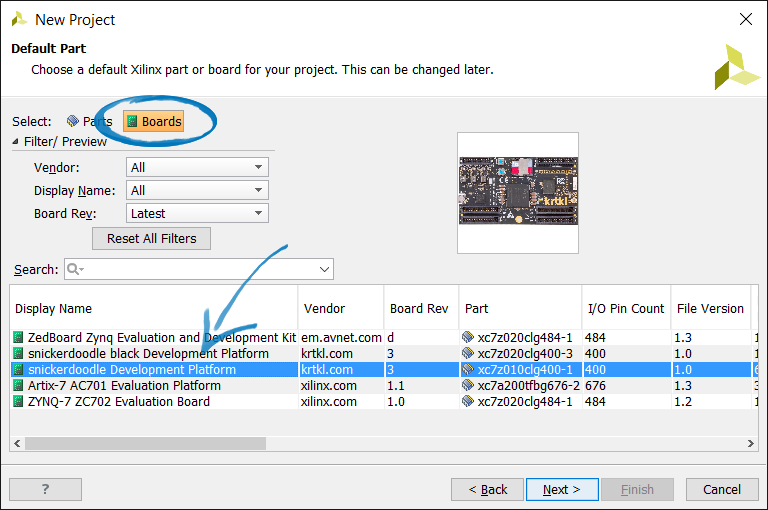
\includegraphics{images/vivado/snickerdoodle_board_select.png}
	\caption{Selecting a Project Board}
	\label{fig:vivadoprojectboard}
\end{figure}


After selecting a board, the details of the project will be listed in the \textit{New Project Summary} shown in \figref{fig:vivadoprojectfinish}. By clicking the "Finish" button, the project will be created and opened in the Vivado graphical user interface (GUI). \\

\begin{figure}
	\centering
	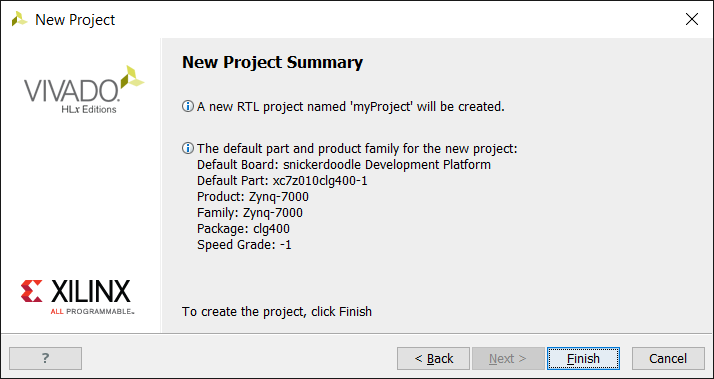
\includegraphics{images/vivado/new_project_summary.png}
	\caption{Review and Finish New Project Creation}
	\label{fig:vivadoprojectfinish}
\end{figure}

% -----------------------------------------------------
% 		Working with Vivado
% -----------------------------------------------------
\section{Working with Vivado}
After creating an empty project, you are free to import existing assets or develop sources from scratch. To get started with development, a block design needs to be created.


%%%-------- Create Block Design ---------
\subsection{Create Block Design}

\begin{marginfigure}
	\centering
	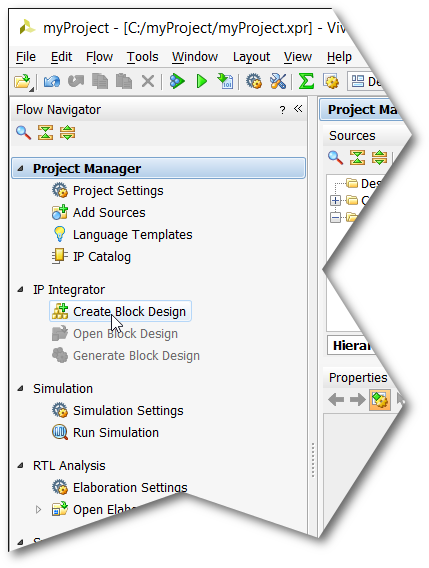
\includegraphics{images/vivado/create_block_diagram.png}
	\caption[Create Block Design]{Create Block Design}
	\label{fig:createblockdesign}
\end{marginfigure}


A block design is a visual representation of the hardware configuration. Hardware configurations can be defined by including or creating sources and assigning hardware I/O. \figref{fig:exampleblockdesign} shows an example block design with hardware definitions for fixed peripherals such as memory interfaces and a some GPIO ports defined in programmable logic. \\


To create a block design for a new project, select \menupath{Flow, Create Block Design} from the menubar or from the "IP Integrator" section of the \textit{Flow Navigator} pane as shown in \figref{fig:createblockdesign}. \\


Adding and integrating sources and IP into a block design can vary greatly depending on the design and application. For additional reading and information on integrating IP can be found at \nocite{xilinxug896:15}. %\url{http://www.xilinx.com/support/documentation/sw_manuals/xilinx2015_4/ug896-vivado-ip.pdf}. 


\clearpage
\begin{figure*}
	\centering
	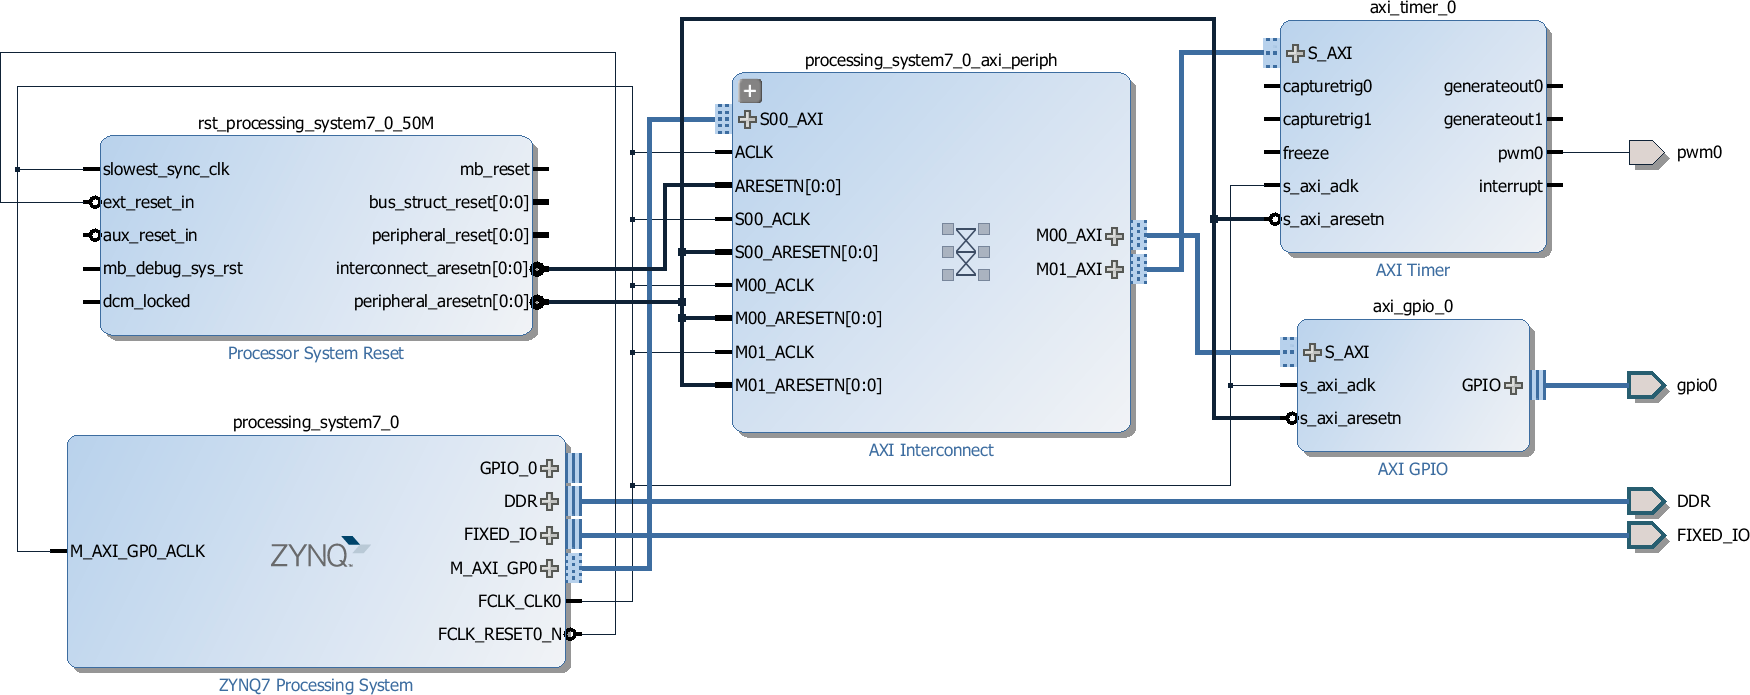
\includegraphics{images/vivado/block_diagram.png}
	\caption[Example Vivado Block Design]{Example Block Design with Zynq Processing System and Microblaze Soft Core Processor}
	\label{fig:exampleblockdesign}
\end{figure*}


\subsection{Create HDL Wrapper}

Before generating a bitstream for the project, an HDL wrapper must be generated for the design. To do this, right click on the design (in this case "base\_design") from within the \textit{Sources} pane and select \menupath{Create HDL Wrapper...}. 


\begin{figure}
	\centering
	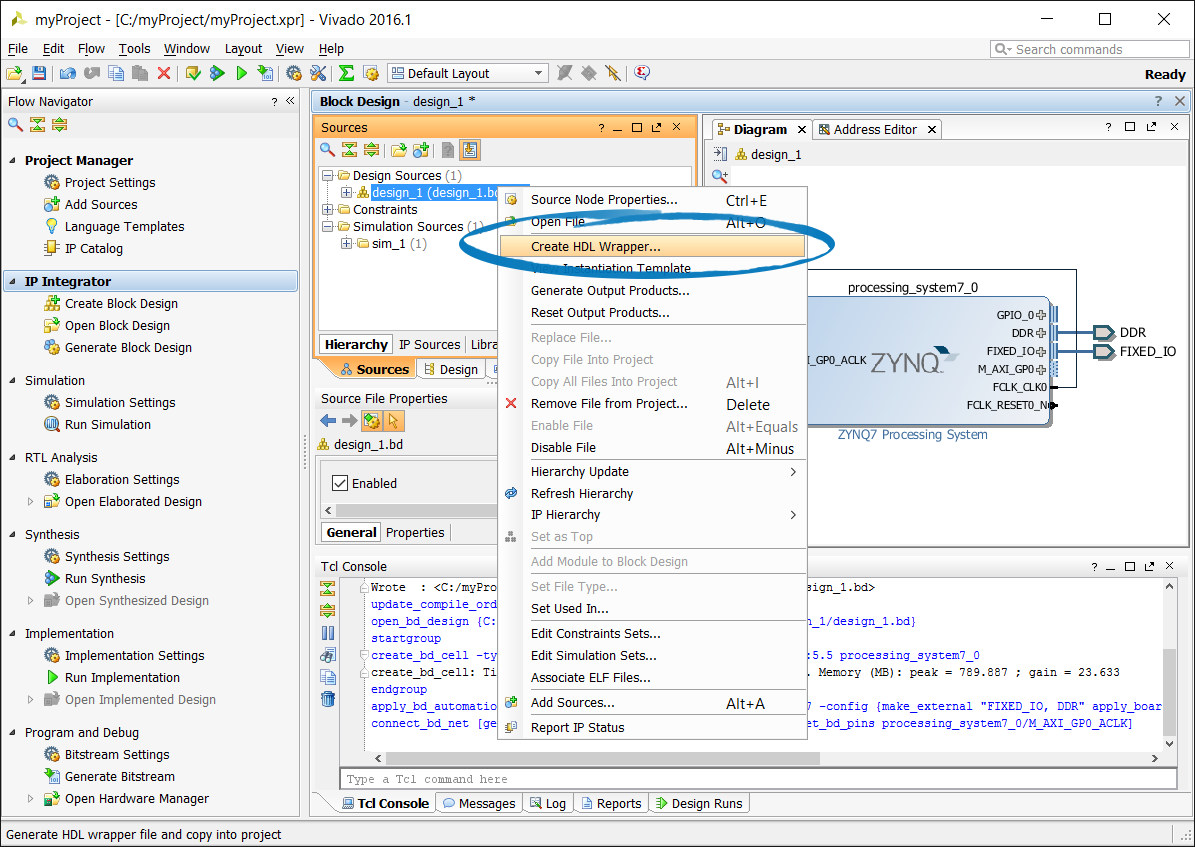
\includegraphics{images/vivado/create_hdl_wrapper.png}
	\caption{Creating an HDL Wrapper for the Design}
	\label{fig:createhdlwrapper}
\end{figure}


%\begin{marginfigure}
%	\centering
%	\includegraphics{images/Create_HDL_Wrapper_Dialog.png}
%	\caption[Create a User Editable or Vivado Auto-Updated HDL Wrapper]{Create a User Editable or Vivado Auto-Updated HDL Wrapper}
%	\label{fig:hdlwrapperdialog}
%\end{marginfigure}





%%%-------- Getting Ports get_ports ----------
\subsection{Getting Ports (\cmdstr{get\_ports})}

After synthesizing and implementing the block design, the \texttt{get\_ports} command can be used in the TCL console to view the ports available to be constrained. Before the synthesis and implementation is complete, the \texttt{get\_ports} command will produce an error message as shown in \lstref{lst:getportserror}.


\begin{lstlisting}[%
	style=text,
	caption={[\texttt{get\_ports} Error Before Synthesis and Implementation]{Error When Getting Ports Before Synthesizing and Implementing Design}},
	label=lst:getportserror
]
> get_ports
ERROR: [Common 17-53] User Exception: No open design. Please open an elaborated, synthesized or implemented design before executing this command.
\end{lstlisting}


After running synthesis and implementation on the design, the ports can be viewed using the \cmdstr{get\_ports} command inside the TCL console within Vivado. The port names returned by this command can be used as constraints to route the PL defined interfaces to specific pins.


\begin{lstlisting}[%
	style=text,
	caption={Example TCL Console Output of \texttt{get\_ports} Command}
]
> get_ports
...
gpio0_tri_io[0] gpio0_tri_io[10] gpio0_tri_io[11]
\end{lstlisting}



%%%-------- Add Sources and IP ---------
\subsection{Add Sources and IP}
\label{sub:addsources}

Adding sources can be done by right clicking inside the \textit{Sources} pane or by selecting \menupath{File, Add Sources...} from the menubar. The \textit{Add Sources Wizard} will appear and allow you to select existing sources, IP and constraints to add to the project.


\begin{figure}
	\centering
	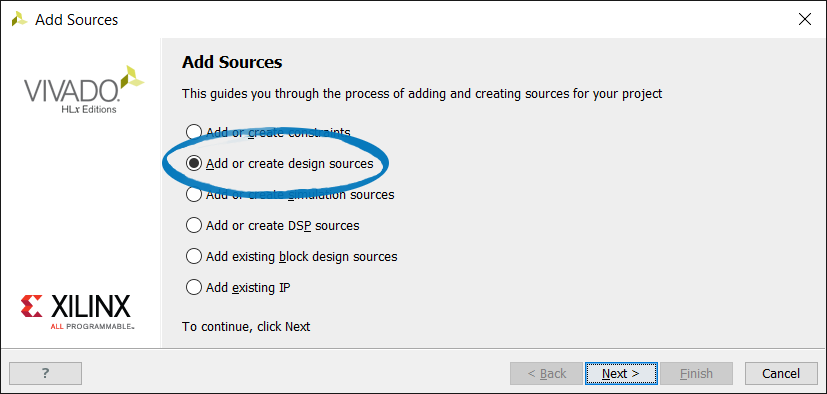
\includegraphics{images/vivado/add_sources.png}
	\caption{Adding New Sources to the Project with the Add Sources Wizard}
	\label{fig:addsourceswiz}
\end{figure}

~\\



%%%-------- Adding Constraints ----------
\subsection{Adding Constraints}
Peripheral interface ports are mapped in the desired FPGA pin using the constraints file. Add a pair of lines to the constraints file for each pin to define the pin/port assignment and the logic level. The logic level should be the same for all pins on a single I/O bank. Connectors JA1 and JA2 share an I/O bank. JB1 and JB2 share an I/O bank. JC1 (on snickerdoodle black) has it's own I/O bank. \\

\begin{marginfigure}
	\centering
	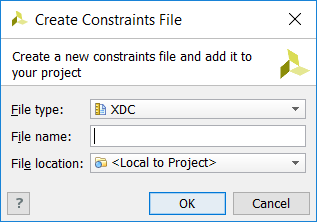
\includegraphics{images/vivado/create_constraints_file.png}
	\caption[Create Constraints File Dialog]{Create Constraints File Dialog}
	\label{fig:createconstraintsfile}
\end{marginfigure}


The \textit{Add Sources Wizard} can be used to create constraints files by selecting \textit{Add or create constraints} and selecting \textit{new file...} and selecting the constraints type and file name as shown in \figref{fig:createconstraintsfile}. An XDC constraints file is essentially a tcl script that sets the system constraints by declaring a set of properties as shown below:


\begin{fullwidth}
\begin{lstlisting}[style=xdc]
###############################################################################
#
#   Constraints file for snickerdoodle black
#
#   Copyright (c) 2016 krtkl inc.
#
###############################################################################
#
#------------------------------------------------------------------------------
# Constraints for GPIO outputs
#------------------------------------------------------------------------------
# JA1 Connector
#------------------------------------------------------------------------------
### JA1.4 (IO_0_35)
set_property PACKAGE_PIN    G14         [get_ports {gpio0_tri_io[24]}]
set_property IOSTANDARD     LVCMOS33    [get_ports {gpio0_tri_io[24]}]

### JA1.5 (IO_L5P_T0_AD9P_35)
set_property PACKAGE_PIN    E18         [get_ports {gpio0_tri_io[8]}]
set_property IOSTANDARD     LVCMOS33    [get_ports {gpio0_tri_io[8]}]

### JA1.6 (IO_L4N_T0_35)
set_property PACKAGE_PIN    D20         [get_ports {gpio0_tri_io[11]}]
set_property IOSTANDARD     LVCMOS33    [get_ports {gpio0_tri_io[11]}]
\end{lstlisting}
\end{fullwidth}



% -----------------------------------------------------
% 		Address Editor
% -----------------------------------------------------
\section{Address Editor}
Hardware interfacing between the processing subsystem and programmable logic can be done through the register space of the hardware block. Each hardware block that requires it, can be assigned a register address space from which the processing subsystem expects to access the hardware. Assigning the register space of a hardware interface is done with the \textit{Address Editor}. In Linux, the offset address assigned to a hardware peripheral will need to be specified for any drivers that are required for control of the peripheral. The specification of the register space and assignment of a driver to the hardware peripheral is done using a node in the device tree. The declaration of the hardware peripheral within the device tree is covered later in this document.

\begin{figure}
	\centering
	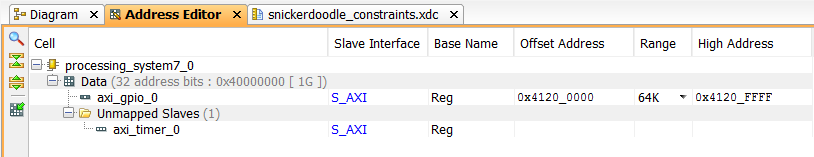
\includegraphics{images/vivado/Address_Editor_Set.png}
	\caption{Unmapped AXI Timer in Address Editor}
	\label{fig:addreditorset}
\end{figure}



\begin{figure}
	\centering
	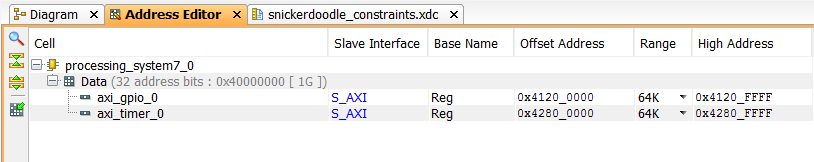
\includegraphics{images/vivado/Address_Editor.png}
	\caption{Address Editor}
	\label{fig:addreditor}
\end{figure}




\subsection{Generating Bitstreams}

Bitstreams can be generated by selecting \menupath{Flow, Generate Bitstream} from the menubar or from within the "Program and Debug" section of the \textit{Flow Navigator} pane as shown in \figref{fig:genbitstream}. The bitstream contains all the information necessary to define the programmable logic and the associated hardware peripherals/interfaces.

\begin{marginfigure}
	\centering
	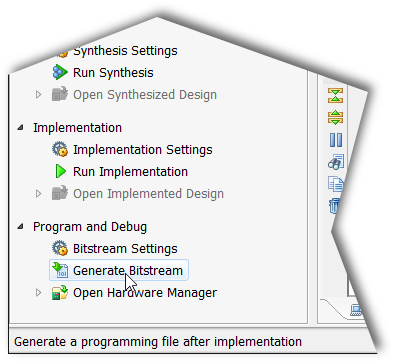
\includegraphics{images/vivado/generate_bitstream.png}
	\caption[Generate Bitstream from Vivado Flow Navigator]{Generate Bitstream from Vivado Flow Navigator}
	\label{fig:genbitstream}
\end{marginfigure}


\section{Exporting Design with SDK}

\subsection{Export the Hardware Platform}

Designs that are implemented using Vivado can be exported and opened in the SDK directly from Vivado. Before a design can be opened in the SDK, the hardware profile must be exported which can be done by selecting \menupath{File, Export, Export Hardware...} from the menubar. \\


\begin{figure}
	\centering
	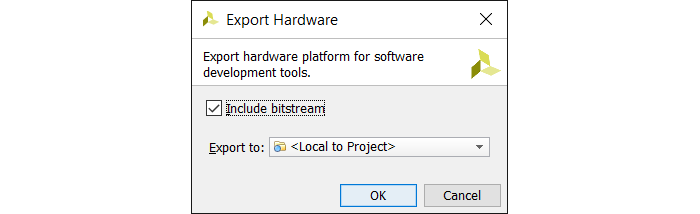
\includegraphics{images/vivado/export_dialog.png}
	\caption{Export Hardware for Software Development Dialog}
	\label{fig:exporthardwaredialog}
\end{figure}

\margininfonote{If you choose an export location other than \texttt{<Local to Project>}, the SDK will need to be launched separately from Vivado to access the exported workspace location}


\figref{fig:exporthardwaredialog} shows the options for hardware export. Select the "Include bitstream" checkbox to include the bitstream with the hardware definition files for use with the SDK. If you would like to use the hardware platform in a workspace other than the hardware project directory, change the selection of the "Export to:" input. This will be the workspace for the SDK. \\




\subsection{Launching the SDK}

The SDK can be launched directly from Vivado to use the exported hardware profile for software development. To launch the SDK from Vivado, select \menupath{File, Launch SDK} from the menubar. If the hardware platform was exported to a directory within the Vivado project (by selecting \texttt{<Local to Project>} as export location), the hardware platform will be immediately available within the SDK workspace. If the hardware was exported to a different directory, you will need to change the workspace directory after the SDK has launched.
